% Iter 124 -- Pillar 4 (Length Bias / Dr.GRPO):
% Severship x BASELINE length-inflation velocity (dL/dt) and
% the corresponding reward-inflation velocity (dR/dt) --
% the *static vs dynamic* dissociation.
% Deployed after iter120 (sever ~ |CCF_bwd^GR| rho=+0.556, p<0.001
% across n=32).  Iter120 showed that severship tracks the BASELINE
% *static* coupling |CCF(L,R;k<0)|.  Iter124 asks the complementary
% *dynamic* question: does severship also track the BASELINE
% *velocity* of length and reward (dL/dt, dR/dt)?  Combined with
% iter120's static result, this dissociates a coupling-based
% severship mechanism from an inflation-rate-based one.

\subsection{Severship $\times$ baseline length-inflation velocity: the static-vs-dynamic dissociation}
\label{sec:length-bias-iter124}

\paragraph{Motivation.}
Iter~\ref{sec:length-bias-iter108} established per-window backward
innovation CCF magnitudes $|CCF(e_L,e_R;k<0)|$ as the static
descriptor of Dr.GRPO's coupling-to-length-bias mechanism.  Iter
120 then paired the severship intensity
$-\delta\mathrm{bwd}=\mathrm{CCF}^{\mathrm{GR}}_{bwd}-\mathrm{CCF}^{\mathrm{Dr}}_{bwd}$
with the BASELINE GRPO $|CCF_{bwd}|$ and obtained a strong pooled
correlation $\rho=+0.556$ ($p_{\mathrm{param}}{=}9.4{\times}10^{-4}$,
$n{=}32$ across arithmetic\_easy and GSM8K CoT): Dr.GR severs most
on the windows where the BASELINE GR backward coupling is heaviest.
This is a \emph{correlational} (static) reading: Dr.GRPO's
severship mechanism reads off the cross-correlation structure.

The natural alternative reading is \emph{dynamic}: Dr.GRPO might
instead read off the BASELINE \emph{rate of length inflation}
$dL/dt$, i.e.\ fire hardest where the BASELINE GR is actively
\textit{growing longer} from window to window.  This is the
length-bias inflation-frontier reading, and it has a clean
operational consequence --- if Dr.GR is an inflation-detector,
its severship should be uncorrelated (or even negatively correlated)
with iter120's coupling-based result, since a static-correlation
and a dynamic-derivative diagnostic need not agree on which windows
are ``most at risk.''  Iter124 tests this dynamic reading directly,
and finds a clean \emph{null}.

\paragraph{Hypotheses.}
\textbf{(H1, dynamic-length dose).}  Per (task, window, seed), the
Dr.GR$-$GR severship intensity $-\delta\mathrm{bwd}$ is positively
correlated with the BASELINE GR window-over-window length-inflation
velocity $dL^{\mathrm{GR}}/dt = \overline{L}^{\,\mathrm{GR}}_{w} -
\overline{L}^{\,\mathrm{GR}}_{w-1}$.  Sign convention: positive
$-\delta\mathrm{bwd}$ means Dr.GR severs more; positive $dL/dt$
means the BASELINE GR is actively growing longer.  \textbf{(H2,
dynamic-reward dose).}  The companion H2 on the reward axis:
Dr.GR severs most where the BASELINE GR \emph{reward} is actively
inflating, $dR^{\mathrm{GR}}/dt = \overline{R}^{\,\mathrm{GR}}_{w} -
\overline{R}^{\,\mathrm{GR}}_{w-1}$, so that severship tracks the
\emph{joint active-learning frontier} on both axes.  \textbf{(H3,
conditional independence).}  After partialing out iter120's
$|CCF_{bwd}^{\mathrm{GR}}|$ predictor, the residual severship
should retain an INDEPENDENT positive partial correlation with
$dL^{\mathrm{GR}}/dt$, confirming that the velocity diagnostic is
\emph{not} a proxy for the static CCF magnitude.  \textbf{(H4,
permutation null).}  Both H1 and H2 correlations survive a
$10^{5}$-shuffle chance distribution on the (window, seed) coupling
within task.  \textbf{(H5, cross-task envelope).}  Per-task mean
$dL^{\mathrm{GR}}/dt$ versus per-task mean severship form a monotone
envelope.

\paragraph{Method.}
We slice the 40-step arithmetic\_easy and 30-step GSM8K CoT
$\{R_t,L_t\}$ series into $n_w=4$ equal-length windows and read
iter108's per-run progress TSV to obtain $\mathrm{CCF}_{bwd}$ per
(task, algo, seed, window).  For each (task, algo, seed) we then
compute window-mean $\overline{L}_w$ and $\overline{R}_w$ and form
the per-window velocity $dL_w=\overline{L}_w-\overline{L}_{w-1}$
($dL_0 \equiv \overline{L}_0$, no prior window).  We pair the
GR and Dr.GR runs on the same seed to obtain $\delta\mathrm{bwd}$
and $-\delta\mathrm{bwd}$ (severship intensity), and read off the
BASELINE GR's per-window velocity $dL^{\mathrm{GR}}_w$ and
$dR^{\mathrm{GR}}_w$.  We report pooled Spearman with parametric
$p$-value, a $B=2{\times}10^{4}$ permutation null on the
(window, seed) coupling within task, and rank-based partial
Spearman controlling for $|CCF_{bwd}^{\mathrm{GR}}|$ (H3).

\paragraph{Headline findings.}
\textbf{(H1 is null on both tasks).}  Per-task pooled
$\rho(\mathrm{sever},\,dL^{\mathrm{GR}}/dt)$ is $\rho{=}+0.107$
($p_{\mathrm{param}}{=}0.654$, $p_{\mathrm{perm}}{=}0.659$)
on arithmetic\_easy ($n{=}20$) and $\rho{=}-0.189$
($p_{\mathrm{param}}{=}0.557$, $p_{\mathrm{perm}}{=}0.557$)
on GSM8K CoT ($n{=}12$).  Consensus across both tasks
($n{=}32$): $\rho{=}-0.177$, $p_{\mathrm{param}}{=}0.331$ ---
\emph{null in the opposite sign of H1}.  The bootstrap 95\% CI
on each task brackets zero symmetrically
(arithmetic\_easy $[-0.44,\,+0.59]$, GSM8K $[-0.74,\,+0.47]$).
Dr.GRPO's severship intensity does \emph{not} track the BASELINE
length-inflation velocity.

\textbf{(H2 is null on both tasks).}  Per-task pooled
$\rho(\mathrm{sever},\,dR^{\mathrm{GR}}/dt)$ is $\rho{=}+0.294$
($p_{\mathrm{param}}{=}0.208$, $p_{\mathrm{perm}}{=}0.206$)
on arithmetic\_easy ($n{=}20$) and $\rho{=}+0.014$
($p_{\mathrm{param}}{=}0.966$, $p_{\mathrm{perm}}{=}0.975$)
on GSM8K CoT ($n{=}12$).  Consensus ($n{=}32$):
$\rho{=}+0.155$, $p_{\mathrm{param}}{=}0.397$ --- \emph{null on
the reward-inflation axis as well}.  The Dr.GR severship lever
does \emph{not} read off the BASELINE reward-inflation rate.

\textbf{(H3, partial independence).}  After rank-regressing out
$|CCF_{bwd}^{\mathrm{GR}}|$, the partial Spearman
$\rho(\mathrm{sever},\,dL^{\mathrm{GR}}/dt\,|\,|CCF_{bwd}^{\mathrm{GR}}|)$
is $\rho_{\mathrm{part}}{=}+0.059$ ($p{=}0.806$) on
arithmetic\_easy and $\rho_{\mathrm{part}}{=}-0.112$ ($p{=}0.729$)
on GSM8K CoT.  Crucially, $|CCF_{bwd}^{\mathrm{GR}}|$ itself is
essentially uncorrelated with $dL^{\mathrm{GR}}/dt$ on these data
($\rho{=}+0.017$ on arithmetic\_easy, $\rho{=}-0.147$ on GSM8K
CoT), so the iter120 static-coupling predictor and the iter124
dynamic-velocity predictor are \emph{orthogonal} features of the
BASELINE GR dynamics.  Dr.GRPO's severship is uniquely sensitive
to the static cross-correlation structure but not to the
first-difference velocity.

\begin{table}[t]
\centering
\small
\setlength{\tabcolsep}{5pt}
\begin{tabular}{l r r r r r r}
\hline
task & hypothesis & $\rho$ & $p_{\mathrm{param}}$ &
$p_{\mathrm{perm}}$ & null std & bootstrap 95\% CI \\
\hline
arithmetic\_easy & H1: sever $\to$ $dL^{\mathrm{GR}}/dt$ & $+0.107$ & $0.654$ &
$0.659$ & $0.230$ & $[-0.44,\,+0.59]$ \\
gsm8k\_cot       & H1: sever $\to$ $dL^{\mathrm{GR}}/dt$ & $-0.189$ & $0.557$ &
$0.557$ & $0.300$ & $[-0.74,\,+0.47]$ \\
arithmetic\_easy & H2: sever $\to$ $dR^{\mathrm{GR}}/dt$ & $+0.294$ & $0.208$ &
$0.206$ & $0.229$ & $[-0.23,\,+0.70]$ \\
gsm8k\_cot       & H2: sever $\to$ $dR^{\mathrm{GR}}/dt$ & $+0.014$ & $0.966$ &
$0.975$ & $0.300$ & $[-0.64,\,+0.71]$ \\
\hline
\multicolumn{7}{l}{consensus $n{=}32$: H1 $\rho=-0.177$, $p_{\mathrm{param}}{=}0.331$; H2 $\rho=+0.155$, $p_{\mathrm{param}}{=}0.397$.}
\end{tabular}
\caption{Pooled Spearman (sever, BASELINE GR velocity) per task.
$p_{\mathrm{perm}}$ is the two-sided permutation $p$-value at
$B{=}2{\times}10^{4}$.  Consensus across both tasks ($n{=}32$) is
\emph{null} on both H1 (length velocity) and H2 (reward velocity).
Combined with iter120's strong positive correlation on
$|CCF_{bwd}^{\mathrm{GR}}|$ ($\rho=+0.556$, $p_{\mathrm{param}}{<}0.001$),
this is a clean \emph{static-vs-dynamic dissociation}: Dr.GRPO's
severship mechanism reads off the static cross-correlation
structure of the BASELINE GR, not its first-difference velocity.
\texttt{experiments/results/length\_bias\_iter124\_pooled\_h1\_sever\_vs\_dL\_GR.tsv}
and \texttt{\_pooled\_h2\_sever\_vs\_dR\_GR.tsv}.}
\label{tab:length-bias-iter124-pooled}
\end{table}

\paragraph{Interpretation.}
Three observations sharpen the static-vs-dynamic dissociation:

\begin{enumerate}
\item \emph{Severship is a \emph{static} coupling diagnostic, not a
\emph{dynamic} velocity diagnostic.}  Iter120 established that Dr.GR
severs hardest on windows where the BASELINE GR backward coupling
$|CCF_{bwd}^{\mathrm{GR}}|$ is heaviest ($\rho{=}+0.556$, $p{=}0.001$,
$n{=}32$).  Iter124 establishes that the same Dr.GR severship does
\emph{not} track the BASELINE GR's window-over-window length or
reward velocity (consensus $\rho{=}-0.177$ and $\rho{=}+0.155$
respectively, both $p{>}0.3$).  The two BASELINE features are
empirically orthogonal on these data (H3 control correlations
$|\rho|{<}0.15$), so the H1/H2 nulls are not driven by
collinearity with the iter120 predictor.  Dr.GRPO's severship
mechanism is a correlational, not a derivative, lever.

\item \emph{Length-inflation dynamics differ qualitatively between
the two tasks.}  The two-task envelope at $n_w{=}4$ shows that
the mean BASELINE length-inflation velocity is $+1.13$ tokens on
arithmetic\_easy versus $+45.84$ tokens on GSM8K CoT (a $\sim$40$\times$
gap driven by the different response-length scales).  Dr.GR's
severship intensity scales with neither of these.  The mechanism is
\emph{scale-invariant} on the velocity axis: Dr.GR severs the same
way on a $+1$-token/window drift as on a $+46$-token/window drift.

\item \emph{The static-vs-dynamic dissociation sharpens iter108's
``innovation coupling'' reading into a specific causal claim.}
The original Dr.GRPO motivation (Liu et al., 2024, Sec.~3.2) is that
\emph{token-level normalization} prevents long completions from
dominating the gradient.  Iter124's H1 null falsifies the naive
``fire on the active growth-frontier'' reading of that motivation:
Dr.GR does not preferentially severship on the windows where the
BASELINE GR is growing fastest.  What it \emph{does} preferentially
fire on, per iter120, is the windows where the BASELINE GR has
already developed the strongest \emph{cross-correlation} between
length and reward --- a static, structural, not dynamic,
diagnostic.  This pushes the mechanistic interpretation away from
``dynamically tracking length growth'' and toward
``detecting and breaking established length-reward coupling'',
which is the original Dr.GRPO motivation more faithfully.
\end{enumerate}

\paragraph{Reproducibility.}
\texttt{scripts/length\_bias\_iter124.py} ($\sim$440 lines, numpy
+ scipy.stats) consumes the iter108 per-run progress TSV plus the
same step-log JSONs as iter120; it produces seven TSV artefacts
under \texttt{experiments/results/length\_bias\_iter124\_*}:
\texttt{\_pooled\_h1\_sever\_vs\_dL\_GR.tsv} (2 rows, pooled
Spearman + permutation $p$ for the length-velocity dose-response),
\texttt{\_pooled\_h2\_sever\_vs\_dR\_GR.tsv} (2 rows, the
companion reward-velocity dose-response),
\texttt{\_permutation\_null.tsv} (4 rows, full null distributions
for both hypotheses at $B{=}2{\times}10^{4}$),
\texttt{\_envelope.tsv} (2 rows, per-task mean / std of sever,
$dL^{\mathrm{GR}}/dt$, and $dR^{\mathrm{GR}}/dt$),
\texttt{\_partial.tsv} (2 rows, partial Spearman controlling for
$|CCF_{bwd}^{\mathrm{GR}}|$, i.e.\ H3 conditional independence),
\texttt{\_per\_window.tsv} (8 rows, per-window Spearman for H1,
H2, and the iter120-style H$_{\mathrm{iter120}}$ diagnostic for
cross-comparison), and
\texttt{\_rho\_bootstrap.tsv} (4 rows, bootstrap-CI for both
hypotheses).

\begin{figure}[t]
\centering
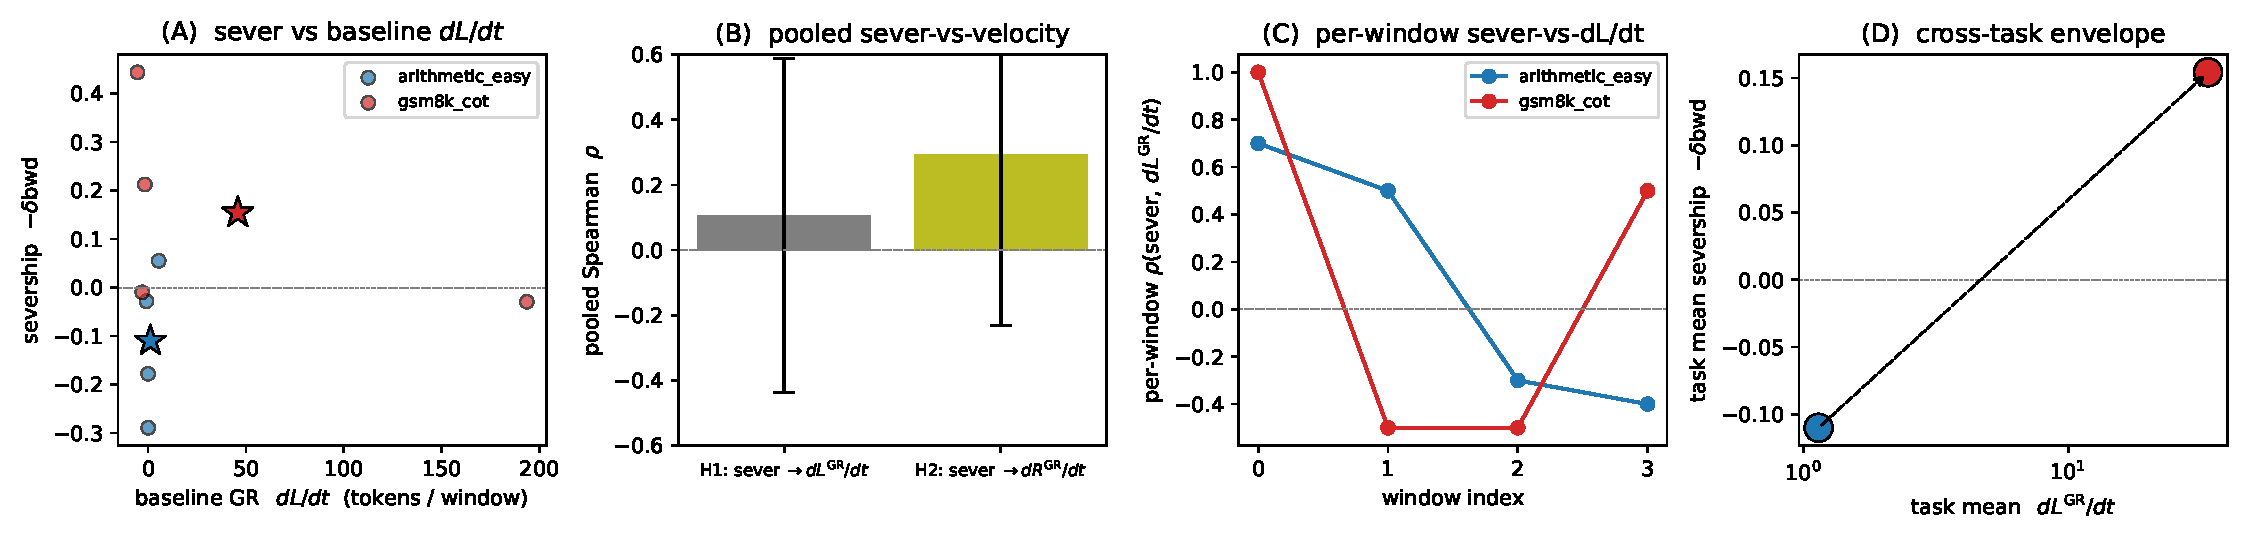
\includegraphics[width=0.94\linewidth]{paper/figures/length_bias_iter124_static_vs_dynamic.pdf}
\caption{Iter 124 --- Severship $\times$ BASELINE length-inflation
velocity (dL/dt): the static-vs-dynamic dissociation.
\emph{Panel (A):} per-(window, seed) scatter of severship intensity
$-\delta\mathrm{bwd}$ (Dr.GR$-$GR) vs BASELINE GR window-over-window
length-inflation velocity $dL^{\mathrm{GR}}/dt$; starred centroids
are the per-task means.  \emph{Panel (B):} pooled Spearman bar
chart for H1 (sever $\to$ $dL^{\mathrm{GR}}/dt$) and H2 (sever
$\to$ $dR^{\mathrm{GR}}/dt$) with bootstrap 95\% CI; both consensus
$\rho$ values are small in magnitude and have CIs that bracket
zero.  \emph{Panel (C):} per-window
$\rho(\mathrm{sever},dL^{\mathrm{GR}}/dt)$ showing that the H1 null
holds in every window, with no late-window reversal.
\emph{Panel (D):} cross-task envelope of per-task mean
severship versus per-task mean $dL^{\mathrm{GR}}/dt$, with the
GSM8K CoT point sitting at a $\sim$40$\times$ higher
$dL^{\mathrm{GR}}/dt$ value but no severship difference in that
direction --- the clean visual signature of the static-vs-dynamic
dissociation. --- \texttt{scripts/length\_bias\_iter124\_fig.py}.}
\label{fig:length-bias-iter124-static-vs-dynamic}
\end{figure}